\begin{figure}


	\centering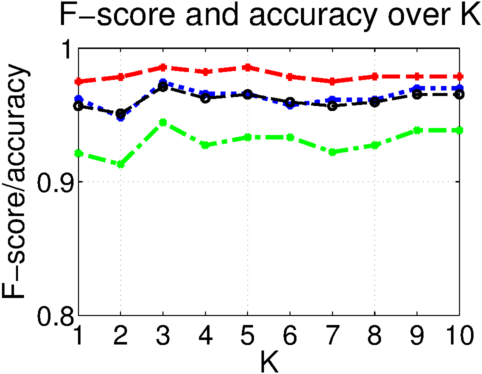
\includegraphics[width=0.3\textwidth]{tex/appendices/test/mfcc2010FP.png}
	\centering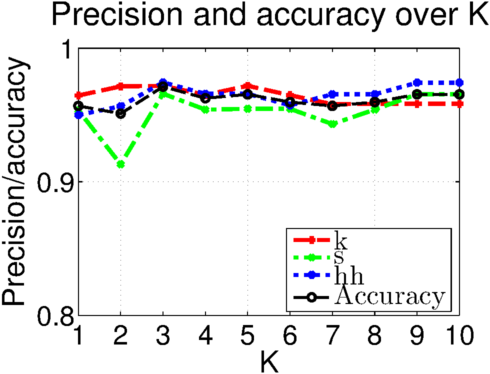
\includegraphics[width=0.3\textwidth]{tex/appendices/test/mfcc2010_P.png}
	\centering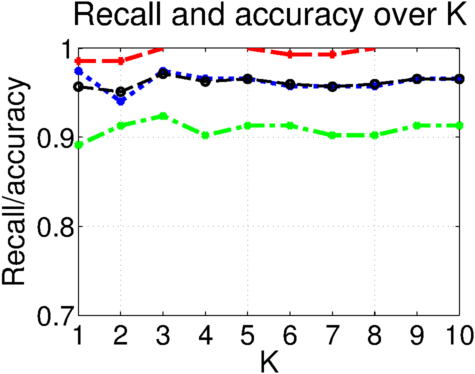
\includegraphics[width=0.3\textwidth]{tex/appendices/test/mfcc2010_R.png}
	
	\caption{Plots over K for MFCC with 20ms windows and 10ms window skips}
\end{figure}
\begin{figure}


	\centering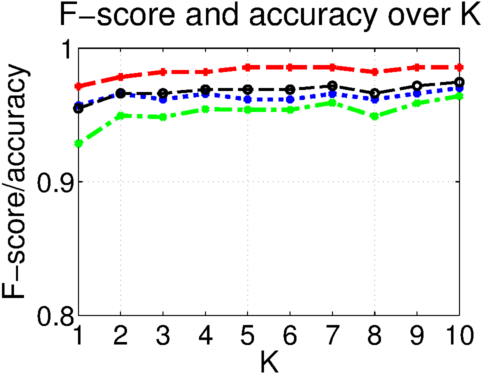
\includegraphics[width=0.3\textwidth]{tex/appendices/test/mfcc105FP.png}
	\centering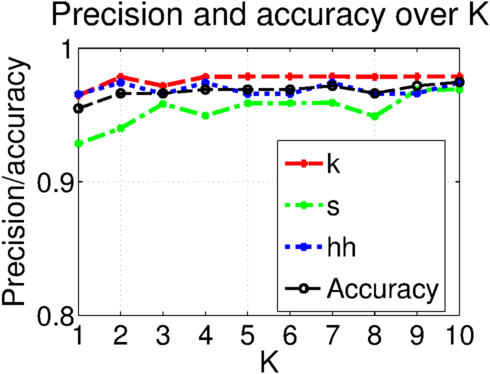
\includegraphics[width=0.3\textwidth]{tex/appendices/test/mfcc105_P.png}
	\centering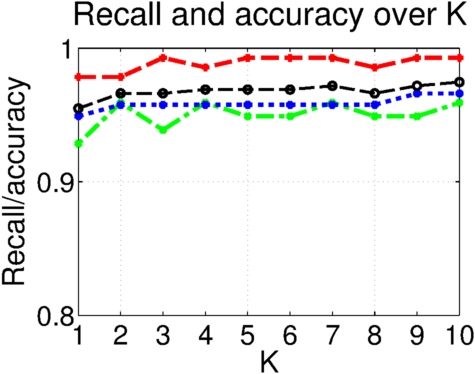
\includegraphics[width=0.3\textwidth]{tex/appendices/test/mfcc105_R.png}
	
	\caption{Plots over K for MFCC with 10ms windows and 5ms window skips}
\end{figure}
\begin{figure}


	\centering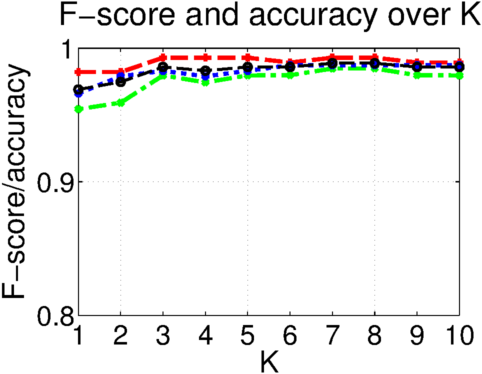
\includegraphics[width=0.3\textwidth]{tex/appendices/test/mfcc52FP.png}
	\centering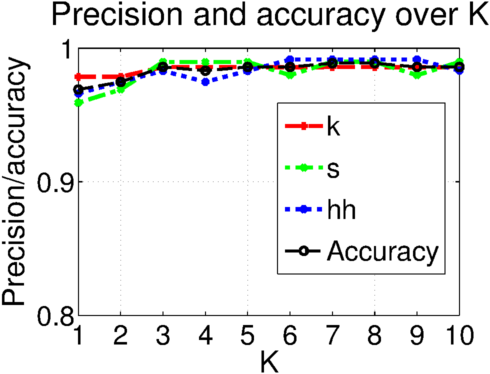
\includegraphics[width=0.3\textwidth]{tex/appendices/test/mfcc52_P.png}
	\centering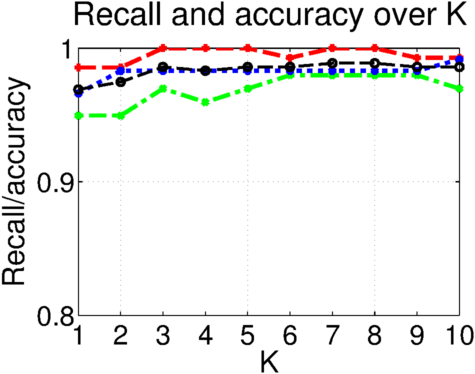
\includegraphics[width=0.3\textwidth]{tex/appendices/test/mfcc52_R.png}
	
	\caption{Plots over K for MFCC with 5ms windows and 2ms window skips}
\end{figure}\clearpage


\begin{table}
\begin{subtable}[tbp]{0.45\textwidth}
\centering
\begin{tabular}{|c|c|c|c"c|}
\cline{2-5}
 \multicolumn{1}{c|}{} & \textbf{k}  & \textbf{s}  & \textbf{hh}  & Prec.\\ \hline
 \textbf{k} & \textcolor{red}{0.986} & 0.054 & 0.000 & 0.965\\ \hline
 \textbf{s} & 0.007 & \textcolor{red}{0.891} & 0.026 & 0.953\\ \hline
 \textbf{hh} & 0.007 & 0.054 & \textcolor{red}{0.974} & 0.950\\ \Xhline{2\arrayrulewidth}
 F & 0.975 & 0.921 & 0.962 & \textcolor{blue}{0.957}\\ \hline
\end{tabular}
\caption{$K=1$}
\end{subtable}
\hfill
\begin{subtable}[tbp]{0.45\textwidth}
\centering
\begin{tabular}{|c|c|c|c"c|}
\cline{2-5}
 \multicolumn{1}{c|}{} & \textbf{k}  & \textbf{s}  & \textbf{hh}  & Prec.\\ \hline
 \textbf{k} & \textcolor{red}{0.986} & 0.043 & 0.000 & 0.971\\ \hline
 \textbf{s} & 0.007 & \textcolor{red}{0.913} & 0.060 & 0.913\\ \hline
 \textbf{hh} & 0.007 & 0.043 & \textcolor{red}{0.940} & 0.957\\ \Xhline{2\arrayrulewidth}
 F & 0.978 & 0.913 & 0.948 & \textcolor{blue}{0.951}\\ \hline
\end{tabular}
\caption{$K=2$}
\end{subtable}
\hfill
\begin{subtable}[tbp]{0.45\textwidth}
\centering
\begin{tabular}{|c|c|c|c"c|}
\cline{2-5}
 \multicolumn{1}{c|}{} & \textbf{k}  & \textbf{s}  & \textbf{hh}  & Prec.\\ \hline
 \textbf{k} & \textcolor{red}{1.000} & 0.043 & 0.000 & 0.972\\ \hline
 \textbf{s} & 0.000 & \textcolor{red}{0.924} & 0.026 & 0.966\\ \hline
 \textbf{hh} & 0.000 & 0.033 & \textcolor{red}{0.974} & 0.974\\ \Xhline{2\arrayrulewidth}
 F & 0.986 & 0.944 & 0.974 & \textcolor{blue}{0.971}\\ \hline
\end{tabular}
\caption{$K=3$}
\end{subtable}
\hfill
\begin{subtable}[tbp]{0.45\textwidth}
\centering
\begin{tabular}{|c|c|c|c"c|}
\cline{2-5}
 \multicolumn{1}{c|}{} & \textbf{k}  & \textbf{s}  & \textbf{hh}  & Prec.\\ \hline
 \textbf{k} & \textcolor{red}{1.000} & 0.054 & 0.000 & 0.965\\ \hline
 \textbf{s} & 0.000 & \textcolor{red}{0.902} & 0.034 & 0.954\\ \hline
 \textbf{hh} & 0.000 & 0.043 & \textcolor{red}{0.966} & 0.966\\ \Xhline{2\arrayrulewidth}
 F & 0.982 & 0.927 & 0.966 & \textcolor{blue}{0.963}\\ \hline
\end{tabular}
\caption{$K=4$}
\end{subtable}
\hfill
\begin{subtable}[tbp]{0.45\textwidth}
\centering
\begin{tabular}{|c|c|c|c"c|}
\cline{2-5}
 \multicolumn{1}{c|}{} & \textbf{k}  & \textbf{s}  & \textbf{hh}  & Prec.\\ \hline
 \textbf{k} & \textcolor{red}{1.000} & 0.043 & 0.000 & 0.972\\ \hline
 \textbf{s} & 0.000 & \textcolor{red}{0.913} & 0.034 & 0.955\\ \hline
 \textbf{hh} & 0.000 & 0.043 & \textcolor{red}{0.966} & 0.966\\ \Xhline{2\arrayrulewidth}
 F & 0.986 & 0.933 & 0.966 & \textcolor{blue}{0.965}\\ \hline
\end{tabular}
\caption{$K=5$}
\end{subtable}
\hfill
\begin{subtable}[tbp]{0.45\textwidth}
\centering
\begin{tabular}{|c|c|c|c"c|}
\cline{2-5}
 \multicolumn{1}{c|}{} & \textbf{k}  & \textbf{s}  & \textbf{hh}  & Prec.\\ \hline
 \textbf{k} & \textcolor{red}{0.993} & 0.043 & 0.009 & 0.965\\ \hline
 \textbf{s} & 0.000 & \textcolor{red}{0.913} & 0.034 & 0.955\\ \hline
 \textbf{hh} & 0.000 & 0.043 & \textcolor{red}{0.957} & 0.957\\ \Xhline{2\arrayrulewidth}
 F & 0.979 & 0.933 & 0.957 & \textcolor{blue}{0.960}\\ \hline
\end{tabular}
\caption{$K=6$}
\end{subtable}
\hfill
\begin{subtable}[tbp]{0.45\textwidth}
\centering
\begin{tabular}{|c|c|c|c"c|}
\cline{2-5}
 \multicolumn{1}{c|}{} & \textbf{k}  & \textbf{s}  & \textbf{hh}  & Prec.\\ \hline
 \textbf{k} & \textcolor{red}{0.993} & 0.054 & 0.009 & 0.958\\ \hline
 \textbf{s} & 0.007 & \textcolor{red}{0.902} & 0.034 & 0.943\\ \hline
 \textbf{hh} & 0.007 & 0.043 & \textcolor{red}{0.957} & 0.966\\ \Xhline{2\arrayrulewidth}
 F & 0.975 & 0.922 & 0.961 & \textcolor{blue}{0.957}\\ \hline
\end{tabular}
\caption{$K=7$}
\end{subtable}
\hfill
\begin{subtable}[tbp]{0.45\textwidth}
\centering
\begin{tabular}{|c|c|c|c"c|}
\cline{2-5}
 \multicolumn{1}{c|}{} & \textbf{k}  & \textbf{s}  & \textbf{hh}  & Prec.\\ \hline
 \textbf{k} & \textcolor{red}{1.000} & 0.054 & 0.009 & 0.958\\ \hline
 \textbf{s} & 0.000 & \textcolor{red}{0.902} & 0.034 & 0.954\\ \hline
 \textbf{hh} & 0.000 & 0.043 & \textcolor{red}{0.957} & 0.966\\ \Xhline{2\arrayrulewidth}
 F & 0.979 & 0.927 & 0.961 & \textcolor{blue}{0.960}\\ \hline
\end{tabular}
\caption{$K=8$}
\end{subtable}
\hfill
\begin{subtable}[tbp]{0.45\textwidth}
\centering
\begin{tabular}{|c|c|c|c"c|}
\cline{2-5}
 \multicolumn{1}{c|}{} & \textbf{k}  & \textbf{s}  & \textbf{hh}  & Prec.\\ \hline
 \textbf{k} & \textcolor{red}{1.000} & 0.054 & 0.009 & 0.958\\ \hline
 \textbf{s} & 0.000 & \textcolor{red}{0.913} & 0.026 & 0.966\\ \hline
 \textbf{hh} & 0.000 & 0.033 & \textcolor{red}{0.966} & 0.974\\ \Xhline{2\arrayrulewidth}
 F & 0.979 & 0.939 & 0.970 & \textcolor{blue}{0.965}\\ \hline
\end{tabular}
\caption{$K=9$}
\end{subtable}
\hfill
\begin{subtable}[tbp]{0.45\textwidth}
\centering
\begin{tabular}{|c|c|c|c"c|}
\cline{2-5}
 \multicolumn{1}{c|}{} & \textbf{k}  & \textbf{s}  & \textbf{hh}  & Prec.\\ \hline
 \textbf{k} & \textcolor{red}{1.000} & 0.054 & 0.009 & 0.958\\ \hline
 \textbf{s} & 0.000 & \textcolor{red}{0.913} & 0.026 & 0.966\\ \hline
 \textbf{hh} & 0.000 & 0.033 & \textcolor{red}{0.966} & 0.974\\ \Xhline{2\arrayrulewidth}
 F & 0.979 & 0.939 & 0.970 & \textcolor{blue}{0.965}\\ \hline
\end{tabular}
\caption{$K=10$}
\end{subtable}
\hfill

\label{tlmfcc2010}

\caption{tcmfcc2010}

\end{table}\clearpage


\begin{table}

\begin{subtable}[tbp]{0.45\textwidth}
\centering
 
\scalebox{0.8}{\begin{tabular}{|c|c|c|c|}\hline
 $K_1$ & $K_2$ & $X^2$ & p\\ \hline
 1 & 2 & 54.000 & 0.02745\\ \hline 
 1 & 3 & 38.250 & 0.14355\\ \hline 
 1 & 4 & 38.250 & 0.14355\\ \hline 
 1 & 5 & 36.000 & 0.05490\\ \hline 
 1 & 6 & 38.250 & 0.14355\\ \hline 
 1 & 7 & 40.500 & 0.27855\\ \hline 
 1 & 8 & 47.250 & 0.09945\\ \hline 
 1 & 9 & 47.250 & 0.09945\\ \hline 
 1 & 10 & 47.250 & 0.09945\\ \hline 
 2 & 3 & 38.250 & 0.14355\\ \hline 
 2 & 4 & 38.250 & 0.14355\\ \hline 
 2 & 5 & 36.000 & 0.05490\\ \hline 
 2 & 6 & 38.250 & 0.14355\\ \hline 
 2 & 7 & 40.500 & 0.27855\\ \hline 
 2 & 8 & 47.250 & 0.09945\\ \hline 
 2 & 9 & 47.250 & 0.09945\\ \hline 
 2 & 10 & 47.250 & 0.09945\\ \hline 
 3 & 4 & 45.000 & 0.00855\\ \hline 
 3 & 5 & 36.000 & 0.01530\\ \hline 
 3 & 6 & 36.000 & 0.07155\\ \hline 
 3 & 7 & 45.000 & 0.03870\\ \hline 
 3 & 8 & 45.000 & 0.03870\\ \hline 
 3 & 9 & 45.000 & 0.03870\\ \hline 
 3 & 10 & 45.000 & 0.03870\\ \hline 
 4 & 5 & 36.000 & 0.01530\\ \hline 
 4 & 6 & 36.000 & 0.07155\\ \hline 
 4 & 7 & 45.000 & 0.03870\\ \hline 
 4 & 8 & 45.000 & 0.03870\\ \hline 
 4 & 9 & 45.000 & 0.03870\\ \hline 
 4 & 10 & 45.000 & 0.03870\\ \hline 
 5 & 6 & 36.000 & 0.01530\\ \hline 
 5 & 7 & 36.000 & 0.05490\\ \hline 
 5 & 8 & 36.000 & 0.05490\\ \hline 
 5 & 9 & 36.000 & 0.05490\\ \hline 
 5 & 10 & 36.000 & 0.05490\\ \hline 
 6 & 7 & 38.250 & 0.14355\\ \hline 
 6 & 8 & 38.250 & 0.14355\\ \hline 
 6 & 9 & 38.250 & 0.14355\\ \hline 
 6 & 10 & 38.250 & 0.14355\\ \hline 
 7 & 8 & 47.250 & 0.09945\\ \hline 
 7 & 9 & 47.250 & 0.09945\\ \hline 
 7 & 10 & 47.250 & 0.09945\\ \hline 
 8 & 9 & 54.000 & 0.02745\\ \hline 
 8 & 10 & 54.000 & 0.02745\\ \hline 
 9 & 10 & 54.000 & 0.02745\\ \hline 

\end{tabular}
} \label{xlmfcc2010}
\caption{xcmfcc2010}
\end{subtable}

\begin{subtable}[tbp]{0.45\textwidth}
\centering
\begin{tabular}{|c|c|c|}
\hline
Class & Amount & Percent\\ \hline
k & 322 & 39.80\\ \hline
s & 214 & 26.45\\ \hline
hh & 273 & 33.75\\ \hline
\end{tabular}
\caption{Training dataset}
\end{subtable}
\hfill
\begin{subtable}[tbp]{0.45\textwidth}
\centering
\begin{tabular}{|c|c|c|}
\hline
Class & Amount & Percent\\ \hline
k & 138 & 39.77\\ \hline
s & 92 & 26.51\\ \hline
hh & 117 & 33.72\\ \hline
\end{tabular}
\caption{Testing dataset}
\end{subtable}
\hfill

\label{dlmfcc2010}

\caption{dcmfcc2010}

\end{table}\clearpage


\begin{table}
\begin{subtable}[tbp]{0.45\textwidth}
\centering
\begin{tabular}{|c|c|c|c"c|}
\cline{2-5}
 \multicolumn{1}{c|}{} & \textbf{k}  & \textbf{s}  & \textbf{hh}  & Prec.\\ \hline
 \textbf{k} & \textcolor{red}{0.978} & 0.031 & 0.017 & 0.965\\ \hline
 \textbf{s} & 0.022 & \textcolor{red}{0.929} & 0.034 & 0.929\\ \hline
 \textbf{hh} & 0.022 & 0.041 & \textcolor{red}{0.949} & 0.966\\ \Xhline{2\arrayrulewidth}
 F & 0.971 & 0.929 & 0.957 & \textcolor{blue}{0.955}\\ \hline
\end{tabular}
\caption{$K=1$}
\end{subtable}
\hfill
\begin{subtable}[tbp]{0.45\textwidth}
\centering
\begin{tabular}{|c|c|c|c"c|}
\cline{2-5}
 \multicolumn{1}{c|}{} & \textbf{k}  & \textbf{s}  & \textbf{hh}  & Prec.\\ \hline
 \textbf{k} & \textcolor{red}{0.978} & 0.010 & 0.017 & 0.978\\ \hline
 \textbf{s} & 0.022 & \textcolor{red}{0.959} & 0.025 & 0.940\\ \hline
 \textbf{hh} & 0.022 & 0.031 & \textcolor{red}{0.958} & 0.974\\ \Xhline{2\arrayrulewidth}
 F & 0.978 & 0.949 & 0.966 & \textcolor{blue}{0.966}\\ \hline
\end{tabular}
\caption{$K=2$}
\end{subtable}
\hfill
\begin{subtable}[tbp]{0.45\textwidth}
\centering
\begin{tabular}{|c|c|c|c"c|}
\cline{2-5}
 \multicolumn{1}{c|}{} & \textbf{k}  & \textbf{s}  & \textbf{hh}  & Prec.\\ \hline
 \textbf{k} & \textcolor{red}{0.993} & 0.020 & 0.017 & 0.972\\ \hline
 \textbf{s} & 0.007 & \textcolor{red}{0.939} & 0.025 & 0.958\\ \hline
 \textbf{hh} & 0.007 & 0.041 & \textcolor{red}{0.958} & 0.966\\ \Xhline{2\arrayrulewidth}
 F & 0.982 & 0.948 & 0.962 & \textcolor{blue}{0.966}\\ \hline
\end{tabular}
\caption{$K=3$}
\end{subtable}
\hfill
\begin{subtable}[tbp]{0.45\textwidth}
\centering
\begin{tabular}{|c|c|c|c"c|}
\cline{2-5}
 \multicolumn{1}{c|}{} & \textbf{k}  & \textbf{s}  & \textbf{hh}  & Prec.\\ \hline
 \textbf{k} & \textcolor{red}{0.986} & 0.010 & 0.017 & 0.979\\ \hline
 \textbf{s} & 0.014 & \textcolor{red}{0.959} & 0.025 & 0.949\\ \hline
 \textbf{hh} & 0.014 & 0.031 & \textcolor{red}{0.958} & 0.974\\ \Xhline{2\arrayrulewidth}
 F & 0.982 & 0.954 & 0.966 & \textcolor{blue}{0.969}\\ \hline
\end{tabular}
\caption{$K=4$}
\end{subtable}
\hfill
\begin{subtable}[tbp]{0.45\textwidth}
\centering
\begin{tabular}{|c|c|c|c"c|}
\cline{2-5}
 \multicolumn{1}{c|}{} & \textbf{k}  & \textbf{s}  & \textbf{hh}  & Prec.\\ \hline
 \textbf{k} & \textcolor{red}{0.993} & 0.010 & 0.017 & 0.979\\ \hline
 \textbf{s} & 0.007 & \textcolor{red}{0.949} & 0.025 & 0.959\\ \hline
 \textbf{hh} & 0.007 & 0.041 & \textcolor{red}{0.958} & 0.966\\ \Xhline{2\arrayrulewidth}
 F & 0.986 & 0.954 & 0.962 & \textcolor{blue}{0.969}\\ \hline
\end{tabular}
\caption{$K=5$}
\end{subtable}
\hfill
\begin{subtable}[tbp]{0.45\textwidth}
\centering
\begin{tabular}{|c|c|c|c"c|}
\cline{2-5}
 \multicolumn{1}{c|}{} & \textbf{k}  & \textbf{s}  & \textbf{hh}  & Prec.\\ \hline
 \textbf{k} & \textcolor{red}{0.993} & 0.010 & 0.017 & 0.979\\ \hline
 \textbf{s} & 0.007 & \textcolor{red}{0.949} & 0.025 & 0.959\\ \hline
 \textbf{hh} & 0.007 & 0.041 & \textcolor{red}{0.958} & 0.966\\ \Xhline{2\arrayrulewidth}
 F & 0.986 & 0.954 & 0.962 & \textcolor{blue}{0.969}\\ \hline
\end{tabular}
\caption{$K=6$}
\end{subtable}
\hfill
\begin{subtable}[tbp]{0.45\textwidth}
\centering
\begin{tabular}{|c|c|c|c"c|}
\cline{2-5}
 \multicolumn{1}{c|}{} & \textbf{k}  & \textbf{s}  & \textbf{hh}  & Prec.\\ \hline
 \textbf{k} & \textcolor{red}{0.993} & 0.010 & 0.017 & 0.979\\ \hline
 \textbf{s} & 0.007 & \textcolor{red}{0.959} & 0.025 & 0.959\\ \hline
 \textbf{hh} & 0.007 & 0.031 & \textcolor{red}{0.958} & 0.974\\ \Xhline{2\arrayrulewidth}
 F & 0.986 & 0.959 & 0.966 & \textcolor{blue}{0.972}\\ \hline
\end{tabular}
\caption{$K=7$}
\end{subtable}
\hfill
\begin{subtable}[tbp]{0.45\textwidth}
\centering
\begin{tabular}{|c|c|c|c"c|}
\cline{2-5}
 \multicolumn{1}{c|}{} & \textbf{k}  & \textbf{s}  & \textbf{hh}  & Prec.\\ \hline
 \textbf{k} & \textcolor{red}{0.986} & 0.010 & 0.017 & 0.979\\ \hline
 \textbf{s} & 0.014 & \textcolor{red}{0.949} & 0.025 & 0.949\\ \hline
 \textbf{hh} & 0.014 & 0.041 & \textcolor{red}{0.958} & 0.966\\ \Xhline{2\arrayrulewidth}
 F & 0.982 & 0.949 & 0.962 & \textcolor{blue}{0.966}\\ \hline
\end{tabular}
\caption{$K=8$}
\end{subtable}
\hfill
\begin{subtable}[tbp]{0.45\textwidth}
\centering
\begin{tabular}{|c|c|c|c"c|}
\cline{2-5}
 \multicolumn{1}{c|}{} & \textbf{k}  & \textbf{s}  & \textbf{hh}  & Prec.\\ \hline
 \textbf{k} & \textcolor{red}{0.993} & 0.010 & 0.017 & 0.979\\ \hline
 \textbf{s} & 0.007 & \textcolor{red}{0.949} & 0.017 & 0.969\\ \hline
 \textbf{hh} & 0.007 & 0.041 & \textcolor{red}{0.966} & 0.966\\ \Xhline{2\arrayrulewidth}
 F & 0.986 & 0.959 & 0.966 & \textcolor{blue}{0.972}\\ \hline
\end{tabular}
\caption{$K=9$}
\end{subtable}
\hfill
\begin{subtable}[tbp]{0.45\textwidth}
\centering
\begin{tabular}{|c|c|c|c"c|}
\cline{2-5}
 \multicolumn{1}{c|}{} & \textbf{k}  & \textbf{s}  & \textbf{hh}  & Prec.\\ \hline
 \textbf{k} & \textcolor{red}{0.993} & 0.010 & 0.017 & 0.979\\ \hline
 \textbf{s} & 0.007 & \textcolor{red}{0.959} & 0.017 & 0.969\\ \hline
 \textbf{hh} & 0.007 & 0.031 & \textcolor{red}{0.966} & 0.974\\ \Xhline{2\arrayrulewidth}
 F & 0.986 & 0.964 & 0.970 & \textcolor{blue}{0.975}\\ \hline
\end{tabular}
\caption{$K=10$}
\end{subtable}
\hfill

\label{tlmfcc105}

\caption{tcmfcc105}

\end{table}\clearpage


\begin{table}

\begin{subtable}[tbp]{0.45\textwidth}
\centering
 
\scalebox{0.8}{\begin{tabular}{|c|c|c|c|}\hline
 $K_1$ & $K_2$ & $X^2$ & p\\ \hline
 1 & 2 & 48.000 & 0.08730\\ \hline 
 1 & 3 & 47.250 & 0.26685\\ \hline   
 1 & 4 & 47.250 & 0.09945\\ \hline 
 1 & 5 & 54.000 & 0.10125\\ \hline 
 1 & 6 & 54.000 & 0.10125\\ \hline 
 1 & 7 & 54.000 & 0.02745\\ \hline 
 1 & 8 & 47.250 & 0.26685\\ \hline 
 1 & 9 & 47.250 & 0.09945\\ \hline 
 1 & 10 & 47.250 & 0.09945\\ \hline 
 2 & 3 & 45.000 & 0.3474\\ \hline 
 2 & 4 & 48.000 & 0.08730\\ \hline 
 2 & 5 & 48.000 & 0.26685\\ \hline 
 2 & 6 & 48.000 & 0.26685\\ \hline 
 2 & 7 & 48.000 & 0.08730\\ \hline 
 2 & 8 & 48.000 & 0.26685\\ \hline 
 2 & 9 & 42.000 & 0.22680\\ \hline 
 2 & 10 & 42.000 & 0.22680\\ \hline 
 3 & 4 & 47.250 & 0.26685\\ \hline 
 3 & 5 & 56.250 & 0.22185\\ \hline 
 3 & 6 & 56.250 & 0.22185\\ \hline 
 3 & 7 & 47.250 & 0.26685\\ \hline 
 3 & 8 & 56.250 & 0.22185\\ \hline 
 3 & 9 & 49.500 & 0.19890\\ \hline 
 3 & 10 & 49.500 & 0.19890\\ \hline 
 4 & 5 & 47.250 & 0.26685\\ \hline 
 4 & 6 & 47.250 & 0.26685\\ \hline 
 4 & 7 & 47.250 & 0.09945\\ \hline 
 4 & 8 & 54.000 & 0.10125\\ \hline 
 4 & 9 & 42.750 & 0.20385\\ \hline 
 4 & 10 & 42.750 & 0.20385\\ \hline 
 5 & 6 & 63.000 & 0.08640\\ \hline 
 5 & 7 & 54.000 & 0.10125\\ \hline 
 5 & 8 & 56.250 & 0.22185\\ \hline 
 5 & 9 & 54.000 & 0.10125\\ \hline 
 5 & 10 & 54.000 & 0.10125\\ \hline 
 6 & 7 & 54.000 & 0.10125\\ \hline 
 6 & 8 & 56.250 & 0.22185\\ \hline 
 6 & 9 & 54.000 & 0.10125\\ \hline 
 6 & 10 & 54.000 & 0.10125\\ \hline 
 7 & 8 & 47.250 & 0.26685\\ \hline 
 7 & 9 & 47.250 & 0.09945\\ \hline 
 7 & 10 & 47.250 & 0.09945\\ \hline 
 8 & 9 & 49.500 & 0.19890\\ \hline 
 8 & 10 & 49.500 & 0.19890\\ \hline 
 9 & 10 & 54.000 & 0.02745\\ \hline 

\end{tabular}
} \label{xlmfcc105}
\caption{xcmfcc105}
\end{subtable}

\begin{subtable}[tbp]{0.45\textwidth}
\centering
\begin{tabular}{|c|c|c|}
\hline
Class & Amount & Percent\\ \hline
k & 326 & 39.23\\ \hline
s & 229 & 27.56\\ \hline
hh & 276 & 33.21\\ \hline
\end{tabular}
\caption{Training dataset}
\end{subtable}
\hfill
\begin{subtable}[tbp]{0.45\textwidth}
\centering
\begin{tabular}{|c|c|c|}
\hline
Class & Amount & Percent\\ \hline
k & 139 & 39.15\\ \hline
s & 98 & 27.61\\ \hline
hh & 118 & 33.24\\ \hline
\end{tabular}
\caption{Testing dataset}
\end{subtable}
\hfill

\label{dlmfcc105}

\caption{dcmfcc105}

\end{table}\clearpage


\begin{table}
\begin{subtable}[tbp]{0.45\textwidth}
\centering
\begin{tabular}{|c|c|c|c"c|}
\cline{2-5}
 \multicolumn{1}{c|}{} & \textbf{k}  & \textbf{s}  & \textbf{hh}  & Prec.\\ \hline
 \textbf{k} & \textcolor{red}{0.986} & 0.020 & 0.008 & 0.979\\ \hline
 \textbf{s} & 0.007 & \textcolor{red}{0.949} & 0.025 & 0.959\\ \hline
 \textbf{hh} & 0.007 & 0.030 & \textcolor{red}{0.966} & 0.966\\ \Xhline{2\arrayrulewidth}
 F & 0.982 & 0.954 & 0.966 & \textcolor{blue}{0.969}\\ \hline
\end{tabular}
\caption{$K=1$}
\end{subtable}
\hfill
\begin{subtable}[tbp]{0.45\textwidth}
\centering
\begin{tabular}{|c|c|c|c"c|}
\cline{2-5}
 \multicolumn{1}{c|}{} & \textbf{k}  & \textbf{s}  & \textbf{hh}  & Prec.\\ \hline
 \textbf{k} & \textcolor{red}{0.986} & 0.020 & 0.008 & 0.979\\ \hline
 \textbf{s} & 0.014 & \textcolor{red}{0.949} & 0.008 & 0.969\\ \hline
 \textbf{hh} & 0.014 & 0.030 & \textcolor{red}{0.983} & 0.975\\ \Xhline{2\arrayrulewidth}
 F & 0.982 & 0.959 & 0.979 & \textcolor{blue}{0.975}\\ \hline
\end{tabular}
\caption{$K=2$}
\end{subtable}
\hfill
\begin{subtable}[tbp]{0.45\textwidth}
\centering
\begin{tabular}{|c|c|c|c"c|}
\cline{2-5}
 \multicolumn{1}{c|}{} & \textbf{k}  & \textbf{s}  & \textbf{hh}  & Prec.\\ \hline
 \textbf{k} & \textcolor{red}{1.000} & 0.010 & 0.008 & 0.986\\ \hline
 \textbf{s} & 0.000 & \textcolor{red}{0.970} & 0.008 & 0.990\\ \hline
 \textbf{hh} & 0.000 & 0.020 & \textcolor{red}{0.983} & 0.983\\ \Xhline{2\arrayrulewidth}
 F & 0.993 & 0.980 & 0.983 & \textcolor{blue}{0.986}\\ \hline
\end{tabular}
\caption{$K=3$}
\end{subtable}
\hfill
\begin{subtable}[tbp]{0.45\textwidth}
\centering
\begin{tabular}{|c|c|c|c"c|}
\cline{2-5}
 \multicolumn{1}{c|}{} & \textbf{k}  & \textbf{s}  & \textbf{hh}  & Prec.\\ \hline
 \textbf{k} & \textcolor{red}{1.000} & 0.010 & 0.008 & 0.986\\ \hline
 \textbf{s} & 0.000 & \textcolor{red}{0.960} & 0.008 & 0.990\\ \hline
 \textbf{hh} & 0.000 & 0.030 & \textcolor{red}{0.983} & 0.975\\ \Xhline{2\arrayrulewidth}
 F & 0.993 & 0.974 & 0.979 & \textcolor{blue}{0.983}\\ \hline
\end{tabular}
\caption{$K=4$}
\end{subtable}
\hfill
\begin{subtable}[tbp]{0.45\textwidth}
\centering
\begin{tabular}{|c|c|c|c"c|}
\cline{2-5}
 \multicolumn{1}{c|}{} & \textbf{k}  & \textbf{s}  & \textbf{hh}  & Prec.\\ \hline
 \textbf{k} & \textcolor{red}{1.000} & 0.010 & 0.008 & 0.986\\ \hline
 \textbf{s} & 0.000 & \textcolor{red}{0.970} & 0.008 & 0.990\\ \hline
 \textbf{hh} & 0.000 & 0.020 & \textcolor{red}{0.983} & 0.983\\ \Xhline{2\arrayrulewidth}
 F & 0.993 & 0.980 & 0.983 & \textcolor{blue}{0.986}\\ \hline
\end{tabular}
\caption{$K=5$}
\end{subtable}
\hfill
\begin{subtable}[tbp]{0.45\textwidth}
\centering
\begin{tabular}{|c|c|c|c"c|}
\cline{2-5}
 \multicolumn{1}{c|}{} & \textbf{k}  & \textbf{s}  & \textbf{hh}  & Prec.\\ \hline
 \textbf{k} & \textcolor{red}{0.993} & 0.010 & 0.008 & 0.986\\ \hline
 \textbf{s} & 0.007 & \textcolor{red}{0.980} & 0.008 & 0.980\\ \hline
 \textbf{hh} & 0.007 & 0.010 & \textcolor{red}{0.983} & 0.991\\ \Xhline{2\arrayrulewidth}
 F & 0.989 & 0.980 & 0.987 & \textcolor{blue}{0.986}\\ \hline
\end{tabular}
\caption{$K=6$}
\end{subtable}
\hfill
\begin{subtable}[tbp]{0.45\textwidth}
\centering
\begin{tabular}{|c|c|c|c"c|}
\cline{2-5}
 \multicolumn{1}{c|}{} & \textbf{k}  & \textbf{s}  & \textbf{hh}  & Prec.\\ \hline
 \textbf{k} & \textcolor{red}{1.000} & 0.010 & 0.008 & 0.986\\ \hline
 \textbf{s} & 0.000 & \textcolor{red}{0.980} & 0.008 & 0.990\\ \hline
 \textbf{hh} & 0.000 & 0.010 & \textcolor{red}{0.983} & 0.991\\ \Xhline{2\arrayrulewidth}
 F & 0.993 & 0.985 & 0.987 & \textcolor{blue}{0.989}\\ \hline
\end{tabular}
\caption{$K=7$}
\end{subtable}
\hfill
\begin{subtable}[tbp]{0.45\textwidth}
\centering
\begin{tabular}{|c|c|c|c"c|}
\cline{2-5}
 \multicolumn{1}{c|}{} & \textbf{k}  & \textbf{s}  & \textbf{hh}  & Prec.\\ \hline
 \textbf{k} & \textcolor{red}{1.000} & 0.010 & 0.008 & 0.986\\ \hline
 \textbf{s} & 0.000 & \textcolor{red}{0.980} & 0.008 & 0.990\\ \hline
 \textbf{hh} & 0.000 & 0.010 & \textcolor{red}{0.983} & 0.991\\ \Xhline{2\arrayrulewidth}
 F & 0.993 & 0.985 & 0.987 & \textcolor{blue}{0.989}\\ \hline
\end{tabular}
\caption{$K=8$}
\end{subtable}
\hfill
\begin{subtable}[tbp]{0.45\textwidth}
\centering
\begin{tabular}{|c|c|c|c"c|}
\cline{2-5}
 \multicolumn{1}{c|}{} & \textbf{k}  & \textbf{s}  & \textbf{hh}  & Prec.\\ \hline
 \textbf{k} & \textcolor{red}{0.993} & 0.010 & 0.008 & 0.986\\ \hline
 \textbf{s} & 0.007 & \textcolor{red}{0.980} & 0.008 & 0.980\\ \hline
 \textbf{hh} & 0.007 & 0.010 & \textcolor{red}{0.983} & 0.991\\ \Xhline{2\arrayrulewidth}
 F & 0.989 & 0.980 & 0.987 & \textcolor{blue}{0.986}\\ \hline
\end{tabular}
\caption{$K=9$}
\end{subtable}
\hfill
\begin{subtable}[tbp]{0.45\textwidth}
\centering
\begin{tabular}{|c|c|c|c"c|}
\cline{2-5}
 \multicolumn{1}{c|}{} & \textbf{k}  & \textbf{s}  & \textbf{hh}  & Prec.\\ \hline
 \textbf{k} & \textcolor{red}{0.993} & 0.010 & 0.008 & 0.986\\ \hline
 \textbf{s} & 0.007 & \textcolor{red}{0.970} & 0.000 & 0.990\\ \hline
 \textbf{hh} & 0.007 & 0.020 & \textcolor{red}{0.992} & 0.983\\ \Xhline{2\arrayrulewidth}
 F & 0.989 & 0.980 & 0.987 & \textcolor{blue}{0.986}\\ \hline
\end{tabular}
\caption{$K=10$}
\end{subtable}
\hfill

\label{tlmfcc52}

\caption{tcmfcc52}

\end{table}\clearpage


\begin{table}

\begin{subtable}[tbp]{0.45\textwidth}
\centering
 
\scalebox{0.8}{\begin{tabular}{|c|c|c|c|}\hline
 $K_1$ & $K_2$ & $X^2$ & p\\ \hline
 1 & 2 & 35.250 & 0.23355\\ \hline 
 1 & 3 & 34.000 & 0.10800\\ \hline 
 1 & 4 & 34.000 & 0.10800\\ \hline 
 1 & 5 & 34.000 & 0.10800\\ \hline 
 1 & 6 & 28.800 & 0.09180\\ \hline 
 1 & 7 & 31.500 & 0.04905\\ \hline 
 1 & 8 & 31.500 & 0.04905\\ \hline 
 1 & 9 & 28.800 & 0.09180\\ \hline 
 1 & 10 & 33.250 & 0.12510\\ \hline 
 2 & 3 & 41.250 & 0.0018\\ \hline 
 2 & 4 & 41.250 & 0.0828\\ \hline 
 2 & 5 & 41.250 & 0.0828\\ \hline 
 2 & 6 & 36.000 & 0.05490\\ \hline 
 2 & 7 & 32.625 & 0.11205\\ \hline 
 2 & 8 & 32.625 & 0.11205\\ \hline 
 2 & 9 & 36.000 & 0.05490\\ \hline 
 2 & 10 & 41.250 & 0.0828\\ \hline 
 3 & 4 & 45.000 & 0.00855\\ \hline 
 3 & 5 & 45.000 & 0.00855\\ \hline 
 3 & 6 & 30.600 & 0.0603\\ \hline 
 3 & 7 & 36.000 & 0.01530\\ \hline 
 3 & 8 & 36.000 & 0.01530\\ \hline 
 3 & 9 & 30.600 & 0.0603\\ \hline 
 3 & 10 & 36.250 & 0.06795\\ \hline 
 4 & 5 & 45.000 & 0.00855\\ \hline 
 4 & 6 & 30.600 & 0.0603\\ \hline 
 4 & 7 & 36.000 & 0.01530\\ \hline 
 4 & 8 & 36.000 & 0.01530\\ \hline 
 4 & 9 & 30.600 & 0.0603\\ \hline 
 4 & 10 & 36.250 & 0.06795\\ \hline 
 5 & 6 & 30.600 & 0.0603\\ \hline 
 5 & 7 & 36.000 & 0.01530\\ \hline 
 5 & 8 & 36.000 & 0.01530\\ \hline 
 5 & 9 & 30.600 & 0.0603\\ \hline 
 5 & 10 & 36.250 & 0.06795\\ \hline 
 6 & 7 & 30.600 & 0.01530\\ \hline 
 6 & 8 & 30.600 & 0.01530\\ \hline 
 6 & 9 & 36.000 & 0.00270\\ \hline 
 6 & 10 & 30.600 & 0.0603\\ \hline 
 7 & 8 & 36.000 & 0.00270\\ \hline 
 7 & 9 & 30.600 & 0.01530\\ \hline 
 7 & 10 & 28.125 & 0.10665\\ \hline 
 8 & 9 & 30.600 & 0.01530\\ \hline 
 8 & 10 & 28.125 & 0.10665\\ \hline 
 9 & 10 & 30.600 & 0.0603\\ \hline 

\end{tabular}
} \label{xlmfcc52}
\caption{xcmfcc52}
\end{subtable}

\begin{subtable}[tbp]{0.45\textwidth}
\centering
\begin{tabular}{|c|c|c|}
\hline
Class & Amount & Percent\\ \hline
k & 326 & 39.14\\ \hline
s & 231 & 27.73\\ \hline
hh & 276 & 33.13\\ \hline
\end{tabular}
\caption{Training dataset}
\end{subtable}
\hfill
\begin{subtable}[tbp]{0.45\textwidth}
\centering
\begin{tabular}{|c|c|c|}
\hline
Class & Amount & Percent\\ \hline
k & 139 & 39.04\\ \hline
s & 99 & 27.81\\ \hline
hh & 118 & 33.15\\ \hline
\end{tabular}
\caption{Testing dataset}
\end{subtable}
\hfill

\label{dlmfcc52}

\caption{dcmfcc52}

\end{table}\clearpage
